\documentclass[12pt]{report} % Increased the font size to 12pt
\usepackage{epigraph}
\usepackage{geometry}

% Optional: customize the style of epigraphs
\setlength{\epigraphwidth}{0.5\textwidth} % Adjust the width of the epigraph
\renewcommand{\epigraphflush}{flushright} % Align the epigraph to the right
\renewcommand{\epigraphrule}{0pt} % No horizontal rule
\usepackage[most]{tcolorbox}
\usepackage{amsmath, amssymb, amsthm}
\usepackage{graphicx}
\usepackage[utf8]{inputenc}
\usepackage{hyperref} % Added for hyperlinks
\usepackage{listings} % Added for code listings
\usepackage{color}    % Added for color definitions
\usepackage[super]{nth}
\usepackage{fancyhdr}
\usepackage{tikz}
\usepackage{cite}
\usetikzlibrary{shapes.geometric, arrows, positioning}

\tikzstyle{startstop} = [rectangle, rounded corners, text centered, draw=black, fill=red!30]
\tikzstyle{io} = [trapezium, trapezium left angle=70, trapezium right angle=110, text centered, draw=black, fill=blue!30]
\tikzstyle{process} = [rectangle, text centered, draw=black, fill=orange!30]
\tikzstyle{decision} = [diamond, text centered, draw=black, fill=green!30]
\tikzstyle{arrow} = [thick,->,>=stealth]

% Define the header and footer for general pages
\pagestyle{fancy}
\fancyhf{} % Clear all header and footer fields
\fancyhead{} % Initially, the header is empty
\fancyfoot[C]{\thepage} % Page number at the center of the footer
\renewcommand{\headrulewidth}{0pt} % No header line on the first page of chapters
\renewcommand{\footrulewidth}{0pt} % No footer line

% Define the plain page style for chapter starting pages
\fancypagestyle{plain}{%
  \fancyhf{} % Clear all header and footer fields
  \fancyfoot[C]{\thepage} % Page number at the center of the footer
  \renewcommand{\headrulewidth}{0pt} % No header line
}

% Apply the 'fancy' style to subsequent pages in a chapter
\renewcommand{\chaptermark}[1]{%
  \markboth{\MakeUppercase{#1}}{}%
}

% Redefine the 'plain' style for the first page of chapters
\fancypagestyle{plain}{%
  \fancyhf{}%
  \fancyfoot[C]{\thepage}%
  \renewcommand{\headrulewidth}{0pt}%
}

% Header settings for normal pages (not the first page of a chapter)
\fancyhead[L]{\slshape \nouppercase{\leftmark}} % Chapter title in the header
\renewcommand{\headrulewidth}{0.4pt} % Header line width on normal pages

\setlength{\headheight}{14.49998pt}
\addtolength{\topmargin}{-2.49998pt}
% Define colors for code listings
\definecolor{codegreen}{rgb}{0,0.6,0}
\definecolor{codegray}{rgb}{0.5,0.5,0.5}
\definecolor{codepurple}{rgb}{0.58,0,0.82}
\definecolor{backcolour}{rgb}{0.95,0.95,0.92}

% Setup for code listings
\lstdefinestyle{mystyle}{
    backgroundcolor=\color{backcolour},
    commentstyle=\color{codegreen},
    keywordstyle=\color{magenta},
    numberstyle=\tiny\color{codegray},
    stringstyle=\color{codepurple},
    basicstyle=\ttfamily\footnotesize,
    breakatwhitespace=false,
    breaklines=true,
    captionpos=b,
    keepspaces=true,
    numbers=left,
    numbersep=5pt,
    showspaces=false,
    showstringspaces=false,
    showtabs=false,
    tabsize=2
}

\lstset{style=mystyle}

% Definition of the tcolorbox for definitions
\newtcolorbox{definitionbox}[1]{
  colback=red!5!white,
  colframe=red!75!black,
  colbacktitle=red!85!black,
  title=#1,
  fonttitle=\bfseries,
  enhanced,
}

% Definition of the tcolorbox for remarks
\newtcolorbox{remarkbox}[1]{
  colback=blue!5!white,     % Light blue background
  colframe=blue!75!black,   % Darker blue frame
  colbacktitle=blue!85!black, % Even darker blue for the title background
  title=#1,            % Title text for remark box
  fonttitle=\bfseries,      % Bold title font
  enhanced,
}

% Definition of the tcolorbox for examples
\newtcolorbox{examplebox}[1]{
  colback=green!5!white,    % Light green background
  colframe=green!75!black,   % Darker green frame
  colbacktitle=green!85!black,  % Even darker green for the title background
  title=#1,         % Title text for example box
  fonttitle=\bfseries,    % Bold title font
  enhanced,
}

% Definitions and examples will be put in these environments
\newenvironment{definition}
    {\begin{definitionbox}}
    {\end{definitionbox}}

\newenvironment{example}
    {\begin{examplebox}}
    {\end{examplebox}}

\geometry{top=1.5in} % Adjust the value as needed
% ----------------------------------------------------------------



\begin{document}

\begin{titlepage}
  \centering
  \vspace*{2cm}
  {\LARGE\bfseries Report for C1 Research Computing Coursework\par}
  \vspace{1cm}
  {\Large\itshape\ CRSiD:\ tmb76\par}
  \vspace{1cm}
  {\Large\itshape\ University of Cambridge\par}
  \vfill
  {\large\today\par}
\end{titlepage}

\tableofcontents

\newpage

\chapter{Introduction}

In this report, an overview of the developping process of a python sudoku solver is given. The aim is to detail the software development of the solver, delving into the experimentation as well as how the code was improved, beyond it functioning as intended. The solver relies on a non-naïve backtracking algorithm. First covered, will be a rational of the choice of solving algorithm and the prototyping of said solver. Then, a larger section will describe the actual development of the code, where the prototyping was wrong, and what solutions were found. This will include profiling, after the solver was finished, to deal with any performance bottlenecks. Beyond the development of the solver, the report will also cover the validation and unit testing of the code, which ensures the code is robust. Finally, the report will cover how the code was packaged and the useability of the solver.


\chapter{Solving Algorithm and Prototyping}

\section{Solving a Sudoku Puzzle}

When solving a sudoku using brain-power, one has multiple technics they can use. Most simple is to go through each cell, and using the sudoku constraints, eliminate impossible values, and hopefully find that there exists only one possible value for the cell. Then, if the sudoku is easy enough, a large part of the cells can be filled in this way as finding the solution to one cell may ``unlock'' another and so on. This can be referred to as the candidate-checking method\cite{cornell_sudoku}.
But there usually comes a point where that process is no longer sufficient. From there, a tedious but very useful option is to mark up the possible values of each cell, and then spend a varying amount of time finding impossibilities of some of those possible by picturing future scenarios, similar to chess\cite{cornell_sudoku}. This is where the average human brain has difficulties, and where a computer performs very well.

\section{Backtracking Algorithm}

A backtracking algorithm is the formal name of the process described above\cite{cornell_sudoku}.
In its most naïve form, it can be described as follows:


\begin{definitionbox}{Naïve Backtracking Algorithm for a 9$\times$9 Sudoku}

  \begin{enumerate}
    \item Go through each cell (in a chosen order).
    \item In the current cell, enumerate from 1 to 9, until:
    \subitem{a.} A value is found that is valid.
    \subitem{b.} 9 is reached, and no valid value was found.
    \item In case of 2.a., go to the next cell and start again from Step 2.
    \item In case of 2.b., go back to the previous cell and, following from Step 2., try the next value.
  \end{enumerate}

\end{definitionbox}

\vspace*{1\baselineskip}
This algorithm has a few advantages. It is a rather simple algorithm to understand, for that reason it should also be relatively simple to implement in code. It offers the guarantee of finding a solution, if one exists, eventually. It can even solve an empty grid, though it will only find one solution out of the 6,670,903,752,021,072,936, 960 possible solutions\cite{cornell_sudoku3}. More on dealing with multiple solutions later.
But being one of the simplest algorithms, there are also reasons why one would use another algorithm. It is a brute-force algorithm, it does not use any heuristics to find the solution faster. It simply iterates through all possible combinations of values, until it finds one that is valid based on the already filled cells. In general, its speed is dependent on the number of empty cells, and the number of possible values for each of those cells. Interestingly, because of it iterating through the above described steps consistently, one can develop a board that is specifically made to be ``difficult'' for this algorithm. In the context of general newspaper sudoku puzzles, it comes down to chance whether the algorithm will be fast or slow. Moreover, it is naïve. This version will test all values from 1 to 9, even when one case may only have 2 possible values. The complexity of the algorithm is then $\mathcal{O}(9^{N_{empty cells}})$, where $N_{empty cells}$ is the number of empty cells in the sudoku. This is a very large number, and so the algorithm is very slow for sudokus with many empty cells.
So rather than wait until it is iterating through the cells, the algorithm could take note of what values are possible for each cell, and then only iterate through those values. This only means doing the validity assessment before the backtracking algorithm, rather than during it. But this means reducing the number of iterations, and so reducing the time it takes to find a solution.

\section{Modified Backtracking Algorithm}


Bringing back our attention to the candidate checking method, we know that we can identify ``obvious'' values for cells, and fill them in. Noting that to do so, we have to mark up the possible values for each cell. We can therefore use a modified backtracking algorithm that uses the candidate checking method prior to backtracking, to reduce the overall complexity of the algorithm (Maximum $\mathcal{O}(N_{v}^{N_{empty cells}})$, where $N_{v}$ is the number of possible value for each cell, and $N_{v}\leq 9$).

\begin{definitionbox}{Modified Backtracking Algorithm with candidate checking for a 9$\times$9 Sudoku}

  \begin{enumerate}
    \item Markup the sudoku with the possible values for each cell.
    \item If the cell has only one possible value, fill it in.
    \item Go back to step 1 and repeat until no more cells can be filled in, i.e.\ the markup does not change.
    \item Start going through each cell (in a chosen order).
    \item In the current cell, enumerate through the possible values for that cell, until:
    \subitem{a.} A value is found that is valid.
    \subitem{b.} All values have been tried and none were valid.
    \item In case of 5.a., go to the next cell and start again from Step 5.
    \item In case of 5.b., go back to the previous cell and, following from Step 5., try the next value.
  \end{enumerate}

\end{definitionbox}

\newpage
\section{Prototyping}


The first idea of what the solver's code would look like was something like this:

\begin{figure}[bthp]
  \centering
  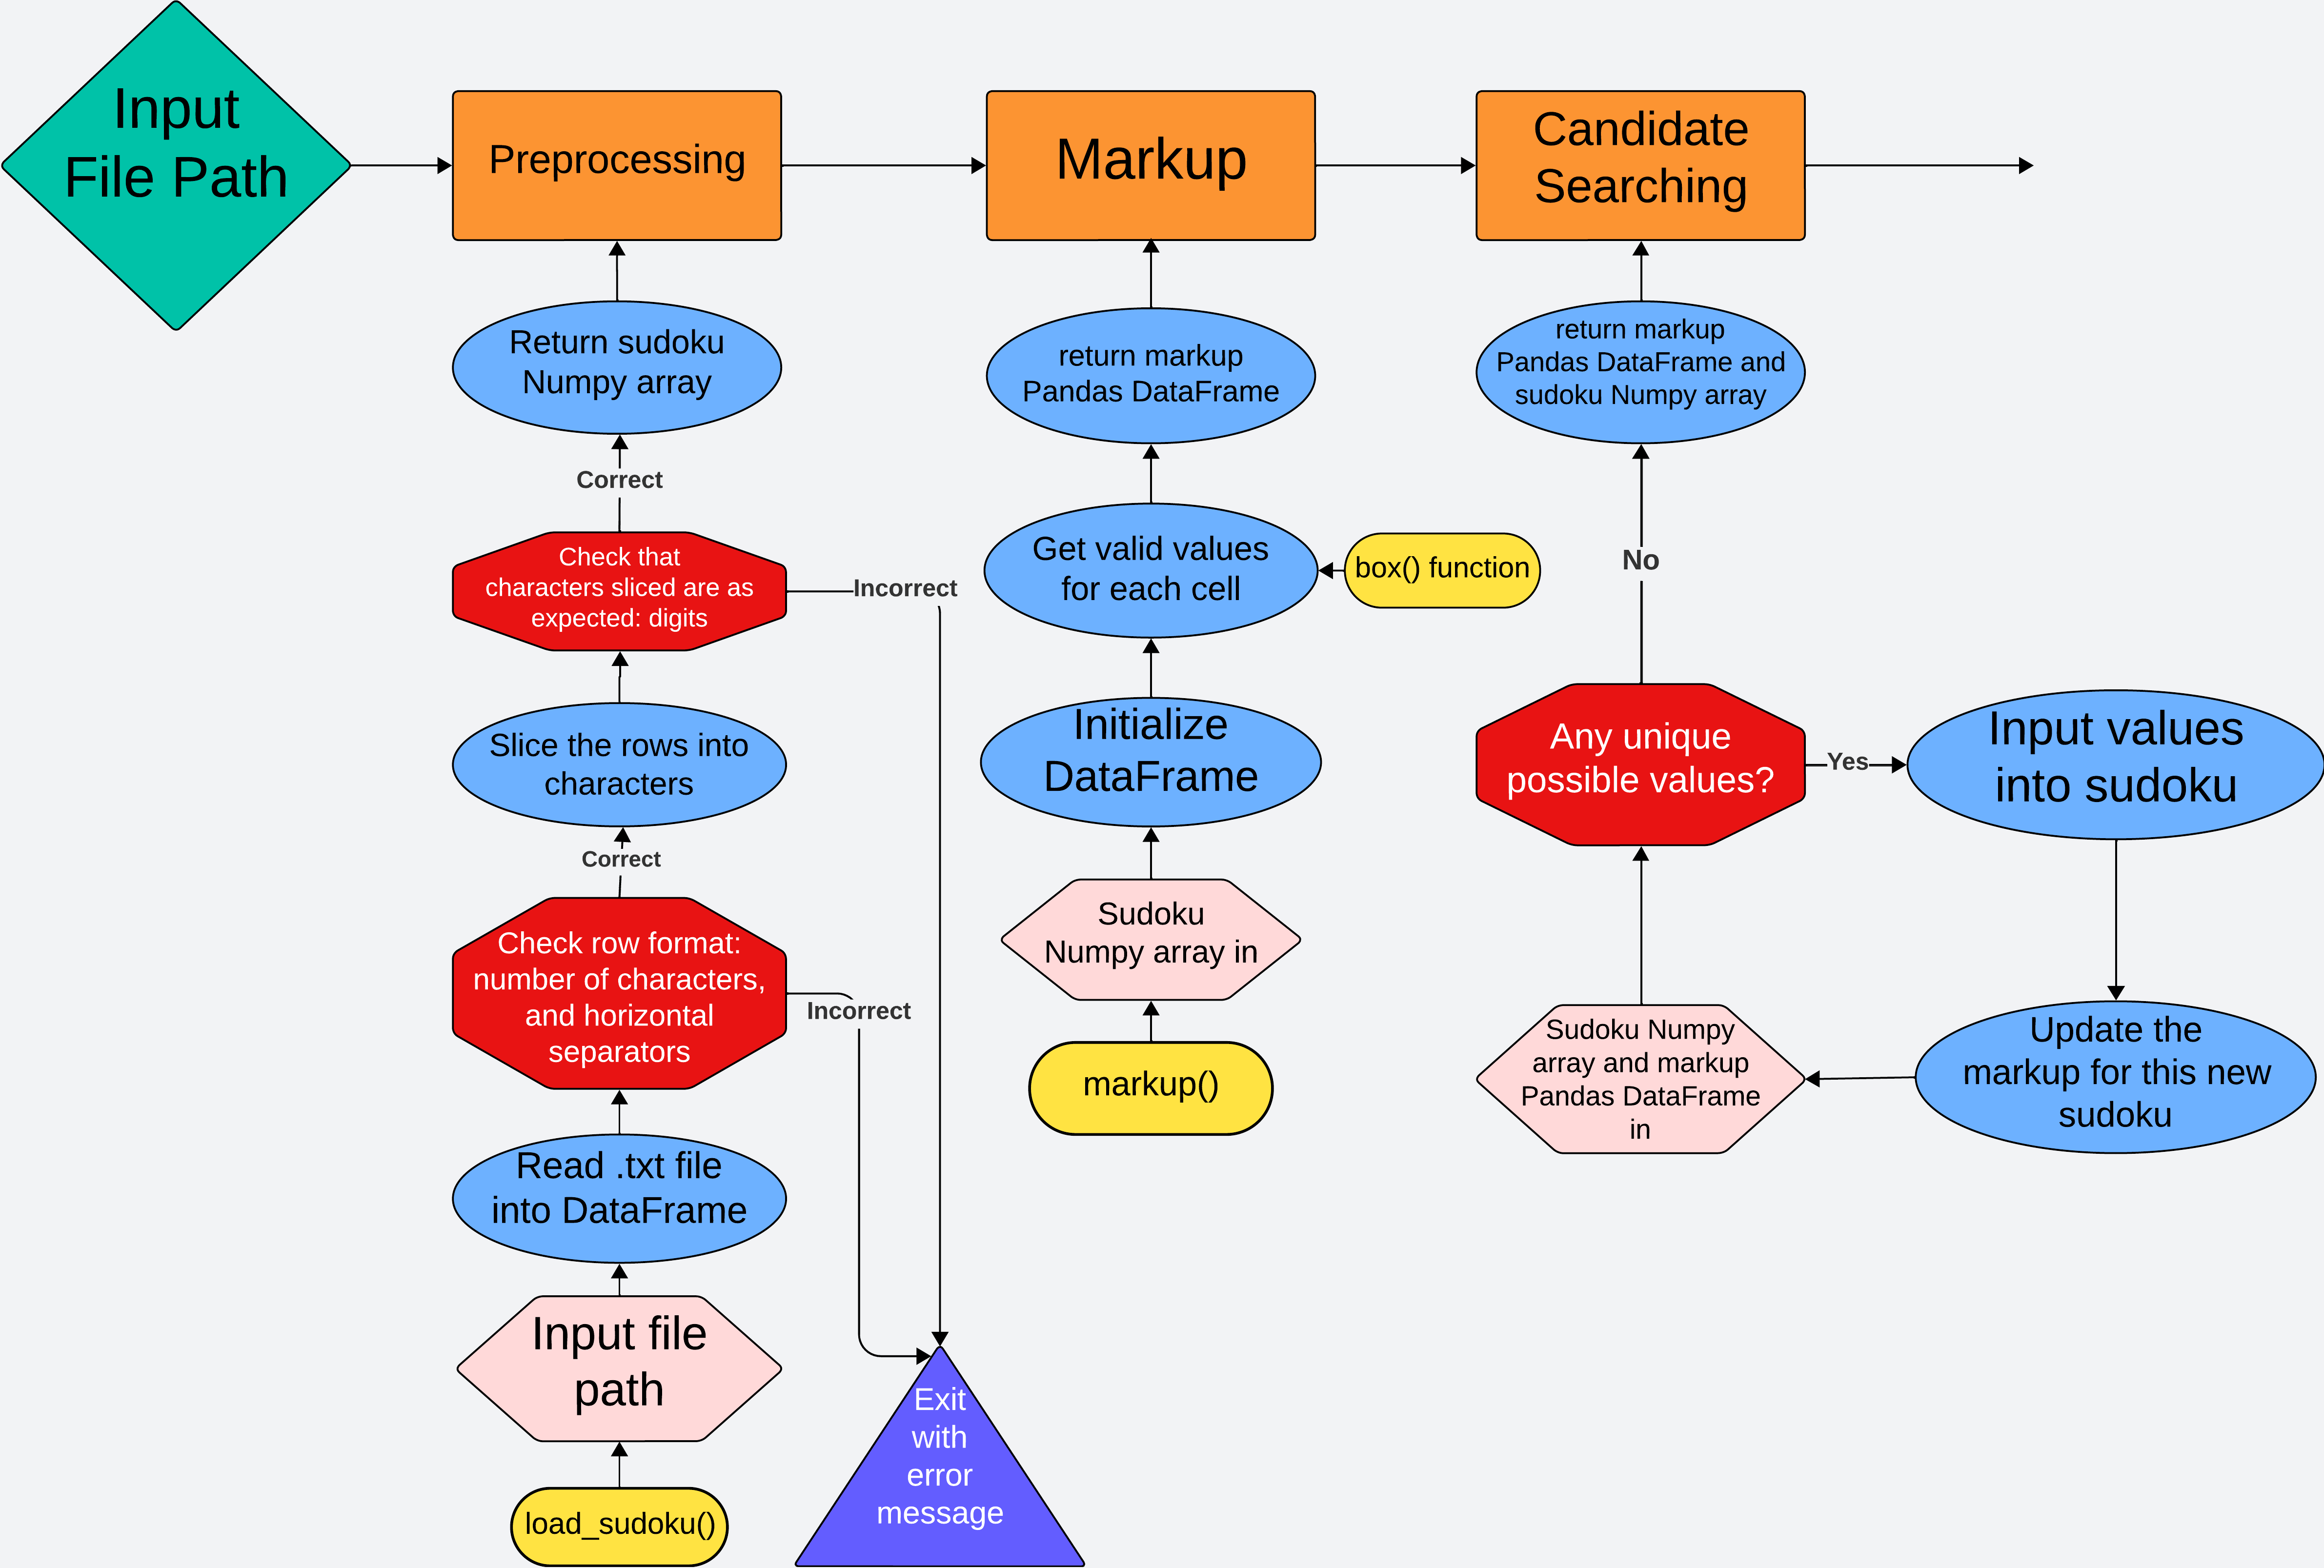
\includegraphics[width=\textwidth]{prototyping1.png}
  \caption{First prototyping of the solver}
\end{figure}

\begin{figure}[bthp]
  \centering
  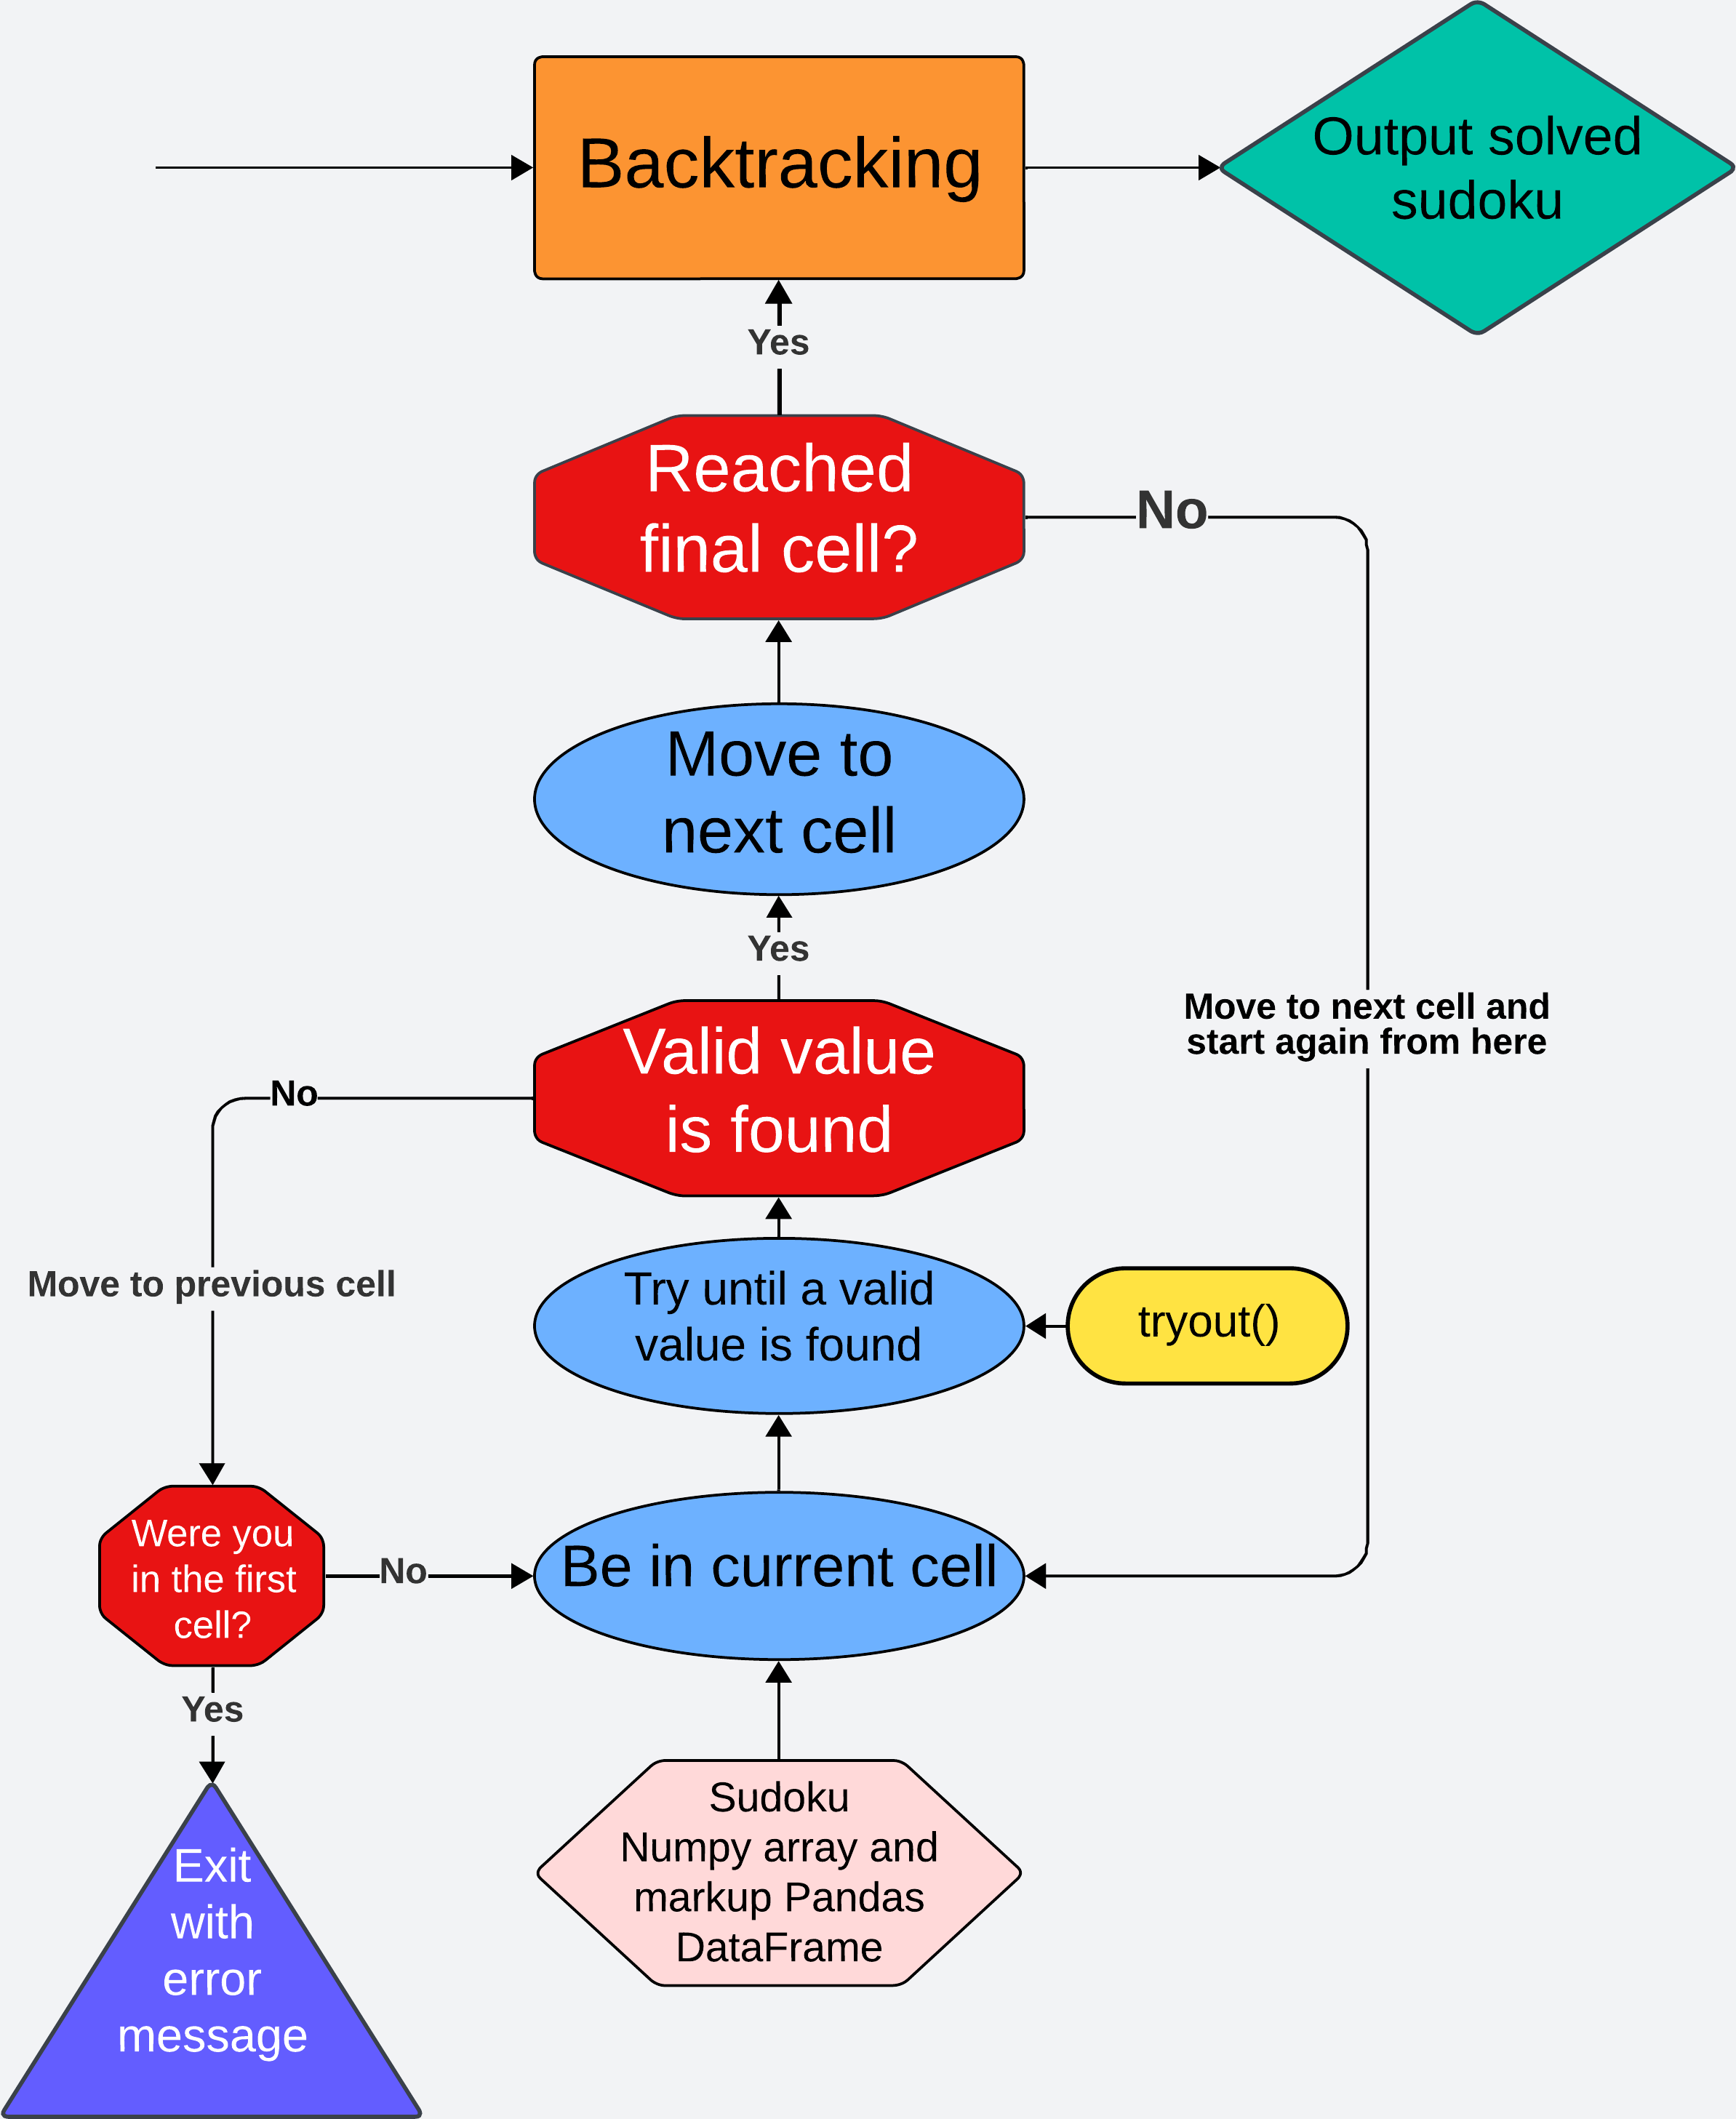
\includegraphics[width=0.8\textwidth]{prototyping1_next.png}
  \caption{First prototyping of the solver (continued)}
\end{figure}

\newpage
The solver would be runnable from the command line like so:

\begin{lstlisting}[language=bash]
  python solve_sudoku.py parameter.ini
\end{lstlisting}

Where the \texttt{parameter.ini} file contains groups of parameters, mainly the input file paths. Which parameters to use would be specified in the main \texttt{solve\_sudoku.py} file. Bearing in mind that the sudokus must be in a \texttt{.txt} file, with the following format, with 0's representing empty cells:

\vspace*{1\baselineskip}
\begin{lstlisting}[language=bash]
  020|000|000
  000|083|400
  090|000|000
  ---+---+---
  000|800|000
  600|009|000
  000|000|093
  ---+---+---
  000|100|000
  000|054|000
  070|000|000
\end{lstlisting}

\vspace*{1\baselineskip}
Using the \texttt{sys} package, the file path would be passed to the \texttt{load\_sudoku()} function, which would read the sudoku from the file path and drop out the separator rows and vertical lines, place the remaining 9 rows of 9 digits into a numpy array. Some checks would be done to ensure the sudoku \texttt{.txt} format is respected. Any infringement would simply make the program stop and print an appropriate error message. There is no point in continuing or trying to correct the mistakes as that could lead to solving a different sudoku than the one the solver's user was intending to solve.
Following this preprocessing step, the markup of the sudoku would be created. The \texttt{markup()} function would simply look at each cell in the sudoku and, applying sudoku rules, determine what values are allowed. It is relatively easy to check the row and the column the cell is in. However, checking the 3$\times$3 box the cell is in is a bit more complicated. For this, a \texttt(box()) function would be created to, given the cell row and column number, return the values of the 3$\times$3 box the cell is in. The \texttt{markup()} function would then use this function to check the box the cell is in. Finally, we use a Pandas DataFrame to put the markup values in, as their number may vary for each cell, and a Pandas DataFrame allows for that, being structure like a dictionary, where a Numpy Array doesn't.
The candidate searching part of the solver would consist of repeating the marking up of the sudoku, inputing of values in cells that only have one possible value, and so on until the markup no longer changes.
Then comes the backtracking part of the solver. Following the steps set out in the modified backtracking algorithm, the solver would go through each cell, and try each possible value for that cell, based on the markup. If it finds a valid one, it goes to the next still empty cell and starts trying out values again. If it doesn't find one, it goes back to the previous cell and tries the next value. If it reaches the end of the possible values for the first cell, it means that the sudoku is unsolvable. The \texttt{tryout()} function would take in the cell location and the markup DataFrame, and return the first valid value it finds. Then it would be placed in a recursive loop that would go through each cell, and try out values until it finds a solution, or until it reaches the end of the possible values for the first cell. The until part would be handled by a \texttt{while} loop, that would check the cell location.
From there the solved sudoku would outputed by printing it to the command line.


\chapter{Development, Experimentation and Profiling}

\section{Development and experimentation}

\subsection{Markup and Box functions}


The \texttt{box()} function was written first to simply split the sudoku into its 9 boxes and return all of them. This would mean unnecessary memory use, so the function was changed to take in the row and column number of the box we wanted (e.g.\ the top right box would be box(1,3)), and return just that one. However, that meant figuring out which box the cell was in, from its coordinates, before calling the \texttt{box} function. Because that would be somewhat messy since the \texttt{box()} function would be called in multiple places, it was then changed to simply take in the cell coordinates and return the box the cell is in.
In its first version, the \texttt{markup()} function would go through each unfilled cell and get the possible values for that cell, putting these in the markup dataframe, at the same coordinates. One problem, which came up when moving on to the candidate checking part of the solver, was that the markup dataframe contained NaN values, for the cells that were already filled. This would cause issues when comparing the markup dataframes when checking if the markup had changed. So, though it was not the most elegant fix, the \texttt{markup()} function was changed to fill in the already filled cells' locations in the markup with those values. In the context of the candidate checking loop, this meant that when updating the sudoku, the values of the cells that were already filled would be overwritten with the same values.

\subsection{Candidate Checking}


To implement the candidate checking method, the markup function simply implemented in a loop whose condition was planned to be that there no longer were any unique possible values in the markup. But with the \texttt{markup()} function changes described above, it was changed to there being no difference between the updated markup and the previous one. Now it was entirely possible that candidate checking was a sufficient method to solve the easier sudokus, in which case an already solved sudoku would be given to the backtracking algorithm. So a break condition was added to the code, to return the solved sudoku if the sudoku no longer had empty ($=0$) cells. Further along the development process, once the solver was working as intended, the \texttt{markup()} function was changed to allow for empty sudokus, giving a warning that there may be multiple solutions when the number of clues at the start of the sudoku is less than 17\cite{cornell_sudoku2}.

\subsection{Backtracking}

Now comes the main part of the solver, the backtracking algorithm. The first attempt consisted of having an embedded \texttt{while} and \texttt{for} loop in which the \texttt{tryout()} function would be used. However, it quickly became obvious this would either need a very convoluted series of loops or simply not be possible. The main issue was how one would be able to go back to the previous iteration of the loop. More precisely, while there is a \texttt{continue} statement to skip to the next iteration, there isn't one to go back one\cite{stackoverflow_python_for_loop}. And though this cited stackoverflow post did provide an approach to have an iterator that could reverse one step, an other issue was the ability to keep track of the values already tried in the previous cell\cite{stackoverflow_python_for_loop}. This would maybe mean having a list to which tried values get added, but this method could lead to code that was hard to follow. Thus, the method settled upon was to use a recursive function structure. The point of a recursive function is that it calls itself within its definition:

\begin{lstlisting}[language=Python]
  def recursive_function(args_1):
    if base_case:
      return something
    else:
      # do something
      recursive_function(args_2)
    # do something
    return something else
\end{lstlisting}

In doing so, the function is called multiple times until a base case condition is fulfilled, a maximum number of recursive depth is reached\cite{stackoverflow_recursion_depth}, or something else depending on what the context and goal of the function is, which stops the recursion. The main benefit, apart from tidiness is that everything outside the function call is kept track of, as expected for the first call but that also means at different recursion levels. For example, the recursive function above could be trying out values for the sudoku. Let's say the first value was tried for \texttt{recursive\_function(args\_1)}, where \texttt{args\_1} would be the first cell, the function would then move on to the line where it calls \texttt{recursive\_function(args\_2)}. Now let's say \texttt{recursive\_function(args\_2)} has tried every possible option it had to try, which could mean having gone down multiple recursive levels, one would exit all recursive levels up to \text{recursive\_function(args\_1)} and be brought back to excatly where they were. The next value for the first cell could be tried and so on. Concisely, the recursive levels are akin to embedded for loops, but without the worry of having to set the number of loops.
Backtracking for solving a sudoku falls under the category of exhaustive search where one tries all possible combinations. Following the Stanford lecture on Exhaustive search and backtracking[slides 13\-17]\cite{stanford_lecture}, this approach can be combined with returning booleans to handle whether to continue the recursion or end it. This gives the following structure:

\begin{examplebox}{Backtracking applied to sudoku}

    \begin{enumerate}
      \item \textbf{If} there are no more decisions to make:
      \subitem{a.}\textbf{Base case} If the sudoku is solved, i.e.\ we've reached the end of the sudoku still-empty cells, end the recursion. Return True.
      \subitem{b.} \textbf{Base case} If the sudoku is not solved, i.e.\ we've gone through every possibility, but there are no more possible values for the last cell, end the recursion. Return False.
      \item \textbf{Else:}
      \subitem{a.} \textbf{Choosing} Iterating over the still empty cells of the sudoku (markup cells with more than one possible value) using a recursive function. Choose a value from the markup cell's list, to which was applied the candidate checking method, to remove values that were no longer valid due to the filling up of the sudoku.
      \subitem{b.} \textbf{Exploring} Input that value in the sudoku, tracking our choice and move to the next cell, starting again at step 1.
      \subitem{c.} \textbf{Unchoosing} If going to the next cell, the valid values list is empty after running the validity check on it, reset the sudoku cell to 0 so that step 2.a.\ works properly, and go back to the previous cell and try the next value (i.e.\ go back to 2.).

    \end{enumerate}

\end{examplebox}



\section{Profiling}

%https://stackoverflow.com/questions/1518346/optimizing-the-backtracking-algorithm-solving-sudoku for the choice to test other orders of backtracking, and for future improvements

%972|853|614
%146|279|538
%583|146|729
%---+---+---
%624|718|953
%817|395|462
%359|462|871
%---+---+---
%798|621|345
%265|934|187
%431|587|296
%Elapsed time: 17843.329435825348 seconds

Having a working solver, profiling was done to identify where time was lost on operations. By running \texttt{cProfile} on our main \texttt{solve\_sudoku.py} file, we got the following output:


\begin{lstlisting}[language=Bash, basicstyle=\tiny]
ncalls  tottime  percall  cumtime  percall filename:lineno(function)
    1    0.000    0.000    0.083    0.083 /src/solve_sudoku.py:25(solve_sudoku 
    3    0.001    0.000    0.051    0.017 /src/solver_tools.py:54(markup)
  237    0.017    0.000    0.027    0.000 /src/solver_tools.py:94(<listcomp>)
318/1    0.001    0.000    0.019    0.019 /src/solver_tools.py:120(backtrack_alg)
  243    0.001    0.000    0.017    0.000 /pandas/core/series.py:1180(__setitem__) 
  279    0.001    0.000    0.014    0.000 /pandas/core/series.py:1396(_maybe_update_cacher)
  317    0.011    0.000    0.014    0.000 /src/solver_tools.py:159(<listcomp>)
  243    0.001    0.000    0.011    0.000 /pandas/core/frame.py:4430(_maybe_cache_changed)
 3282    0.005    0.000    0.009    0.000 /src/preprocessing.py:89(box) 
 3287    0.002    0.000    0.006    0.000 /numpy/core/fromnumeric.py:1768(ravel)
    3    0.002    0.001    0.006    0.002 /src/solver_tools.py:18(check_sudoku)
  279    0.000    0.000    0.006    0.000 /pandas/core/frame.py:3779(_ixs)
  643    0.002    0.000    0.006    0.000 /pandas/core/frame.py:3856(__getitem__)
  243    0.003    0.000    0.005    0.000 /pandas/core/internals/managers.py:1045(iset)
    6    0.000    0.000    0.005    0.001 /pandas/core/frame.py:668(__init__)
    5    0.000    0.000    0.004    0.001 /pandas/core/internals/construction.py:423(dict_to_mgr)
 3287    0.004    0.000    0.004    0.000 {built-in method numpy.asanyarray}
 3282    0.003    0.000    0.003    0.000 /src/preprocessing.py:128(<listcomp>)
  279    0.000    0.000    0.003    0.000 /pandas/core/frame.py:4387(_box_col_values)
  400    0.001    0.000    0.002    0.000 /pandas/core/series.py:1016(__getitem__)
  ....   .....    .....    .....    ..... mostly built-in functions of packages
\end{lstlisting}

As can be seen a large amount of time is lost with the list comprehension lines that are used in order to create the markups, get the valid values from the markup cell in the backtrack algorithm, and when getting the sudoku box, the cell is in. One fix for this is to use sets. Sets are very similar to lists but are unordered and only contain unique values\cite{freecodecamp_python_set_vs_list}. This means that originally, when list comprehension was used to get possible values, the code would check which value was not in a list which potentially contained duplicate, especially zeros which we did not drop. This meant python had to unnecessarily check elements in those lists. Whereas when using sets, the sets of the values in the row, column and box, could be unionized into a single set that would contain a maximum of 10 values, including the 0. The time it took for these value checking lines to be run could then be reduced significantly. The profiling output after this change was:

\begin{lstlisting}[language=Bash, basicstyle=\tiny]
   ncalls  tottime  percall  cumtime  percall filename:lineno(function)
        1    0.000    0.000    0.047    0.047 /src/solve_sudoku.py:26(solve_sudoku)
        3    0.002    0.001    0.027    0.009 /src/solver_tools.py:56(markup)
      243    0.001    0.000    0.017    0.000 /pandas/core/series.py:1180(__setitem__)
      279    0.001    0.000    0.014    0.000 /pandas/core/series.py:1396(_maybe_update_cacher)
      243    0.001    0.000    0.011    0.000 /pandas/core/frame.py:4430(_maybe_cache_changed)
    318/1    0.003    0.000    0.010    0.010 /src/solver_tools.py:147(backtrack_alg)
      279    0.000    0.000    0.005    0.000 /pandas/core/frame.py:3779(_ixs)
      643    0.002    0.000    0.005    0.000 /pandas/core/frame.py:3856(__getitem__)
        3    0.002    0.001    0.005    0.002 /src/solver_tools.py:20(check_sudoku)
        6    0.000    0.000    0.005    0.001 /pandas/core/frame.py:668(__init__)
      243    0.003    0.000    0.005    0.000 /pandas/core/internals/managers.py:1045(iset)
        5    0.000    0.000    0.005    0.001 /pandas/core/internals/construction.py:423(dict_to_mgr)
      279    0.000    0.000    0.003    0.000 /pandas/core/frame.py:4387(_box_col_values)
      400    0.001    0.000    0.002    0.000 /pandas/core/series.py:1016(__getitem__)
     1283    0.002    0.000    0.002    0.000 /src/preprocessing.py:112(box)
     1288    0.001    0.000    0.002    0.000 /numpy/core/fromnumeric.py:1768(ravel)
      317    0.002    0.000    0.002    0.000 /src/solver_tools.py:191(<listcomp>)
5206/3341    0.001    0.000    0.002    0.000 {built-in method builtins.len}
        1    0.000    0.000    0.001    0.001 /pandas/core/frame.py:10039(map)
        1    0.000    0.000    0.001    0.001 /pandas/core/frame.py:9867(apply)
      243    0.000    0.000    0.001    0.000 /pandas/core/series.py:1270(_set_with_engine)
    ....     .....    .....    .....    ..... mostly built-in functions of packages

\end{lstlisting}

It can be seen the cumulative times are much lower, and the time spent on the list comprehension lines is now either negligible or reduced by more than a factor of 10. This was all running for a near-empty sudoku that would make large use of the backtracking algorithm to solve:

\begin{lstlisting}[language=Bash]
000|000|000
001|000|200
000|000|000
---+---+---
000|000|000
000|000|000
000|000|000
---+---+---
000|000|000
000|000|000
000|000|000
\end{lstlisting}

And the time it took to solve this sudoku before the set improvement was 0.049503 seconds, and 0.020695 seconds after the improvement. This was only timing the line where we call the main \texttt{solve\_sudoku()} function, not running the entire file. Now the large amount of pandas functions using a non-negligible of time does bring the question of whether having the markup be updated many times might be an issue when the sudoku has a large enough amount of clues and a good part of it gets solved by the candidate checking method. In summary, maybe the candidate checking method is actually slowing down our solver. We test this now using an easy sudoku which can be solved entirely by the candidate checking method:

\begin{lstlisting}[language=Bash]
002|560|470
058|403|000
004|020|008
---+---+---
781|000|040
409|100|726
006|047|800
---+---+---
007|006|013
005|030|007
060|709|200
\end{lstlisting}


We obtained the following profiling output:

\begin{lstlisting}[language=Bash, basicstyle=\tiny]
          ncalls  tottime  percall  cumtime  percall filename:lineno(function)
          1    0.001    0.001    0.161    0.161 /src/solve_sudoku.py:26(solve_sudoku)
         18    0.005    0.000    0.138    0.008 /src/solver_tools.py:56(markup)
       1458    0.004    0.000    0.098    0.000 /pandas/core/series.py:1180(__setitem__)
       1629    0.005    0.000    0.078    0.000 /pandas/core/series.py:1396(_maybe_update_cacher)
       1458    0.004    0.000    0.063    0.000 /pandas/core/frame.py:4430(_maybe_cache_changed)
       1620    0.003    0.000    0.031    0.000 /pandas/core/frame.py:3779(_ixs)
       1458    0.013    0.000    0.026    0.000 /pandas/core/internals/managers.py:1045(iset)
       2728    0.008    0.000    0.023    0.000 /pandas/core/frame.py:3856(__getitem__)
       1620    0.002    0.000    0.017    0.000 /pandas/core/frame.py:4387(_box_col_values)
         19    0.000    0.000    0.016    0.001 /pandas/core/frame.py:668(__init__)
         19    0.001    0.000    0.015    0.001 /pandas/core/internals/construction.py:423(dict_to_mgr)
26809/15959    0.005    0.000    0.009    0.000 {built-in method builtins.len}
       1620    0.001    0.000    0.008    0.000 /pandas/core/frame.py:656(_constructor_sliced_from_mgr)
       1458    0.001    0.000    0.008    0.000 /pandas/core/series.py:1270(_set_with_engine)
       1620    0.005    0.000    0.007    0.000 /pandas/core/internals/managers.py:991(iget)
       1458    0.002    0.000    0.007    0.000 /pandas/core/series.py:1385(_check_is_chained_assignment_possible)
       1270    0.002    0.000    0.007    0.000 /pandas/core/series.py:1016(__getitem__)
       2728    0.002    0.000    0.006    0.000 /pandas/core/frame.py:4405(_get_item_cache)  
       1458    0.001    0.000    0.006    0.000 /pandas/core/internals/managers.py:1977(setitem_inplace)
       1639    0.004    0.000    0.005    0.000 /pandas/core/generic.py:6147(__finalize__)
       5456    0.004    0.000    0.005    0.000 /pandas/core/indexing.py:2678(check_dict_or_set_indexers)
47346/47327    0.004    0.000    0.005    0.000 {built-in method builtins.isinstance}
       4186    0.003    0.000    0.005    0.000 /pandas/core/indexes/range.py:394(__contains__)
          3    0.002    0.001    0.005    0.002 /src/solver_tools.py:20(check_sudoku)
       ....    .....    .....    .....    ..... mostly built-in functions of packages
\end{lstlisting}

Running the solver for this sudoku, it found a solution in 0.05651 seconds but did so much quicker in 0.00988 seconds when only getting the markup file once and not updating it. Unfortunately, our first assumption which was that conducting a candidate check to get rid of obvious values would be reducing the time spent using the backtracking method

\subsection*{Future improvements}

Apart from the obvious complete change of solving algorithm for better performance, there are a few future improvements that could be tested. 

Possibly using a different library than pandas\cite{no_copy_dataframe}


\chapter{Validation, Unit Tests and CI set up}

\section{Validation}

A check\_sudoku function was written to check that the sudoku is valid. It checks that each row, column and box, and that there are no duplicates.

\section{Unit Tests}

\section{CI set up}

\chapter{Packaging and Usability}

\section{Packaging}

\section{Usability}


\chapter{Summary}

\bibliographystyle{plain}
\bibliography{refs.bib}

\end{document}
